\begin{multicols}{2}
\byline{Мажоретките на ГПНЕ’’Гьоте’’}{Пламена Иванова, 10 клас}
Мажоретният състав на ГПНЕ’’Гьоте’’ е основан през 2005 година във връзка с 45 
годишнината на училището по идея на госпожа Мария Каравасилева. Те са първите в 
гимназиален курс. През 2006 г. са поканени в София по повод 24 май. Взимат 
участие в шествието на всички мажоретни състави, както и оркестъра на ПГМЕ - 
Професионална гимназия по механоелектротехника и електроника. След тази изява 
министърът на просветата Даниел Вълчев изпраща благодарствено писмо на Немската 
гимназия. Първият капитан на състава е Илияна Михайлова,нейни последователки - 
Люба Пантелеева, Силвия Капитанова (благодарение на която мажореките участват 
във фестивала в Турция по случай 6 декември) , Мирела Паздерова и Калина 
Казанджиева. Мажоретките и до днес продължават да се развиват, всяка година има 
кастинг за нови,желаещи да танцуват и да представят достойно гимназията 
момичета.

\end{multicols}

\begin{center}
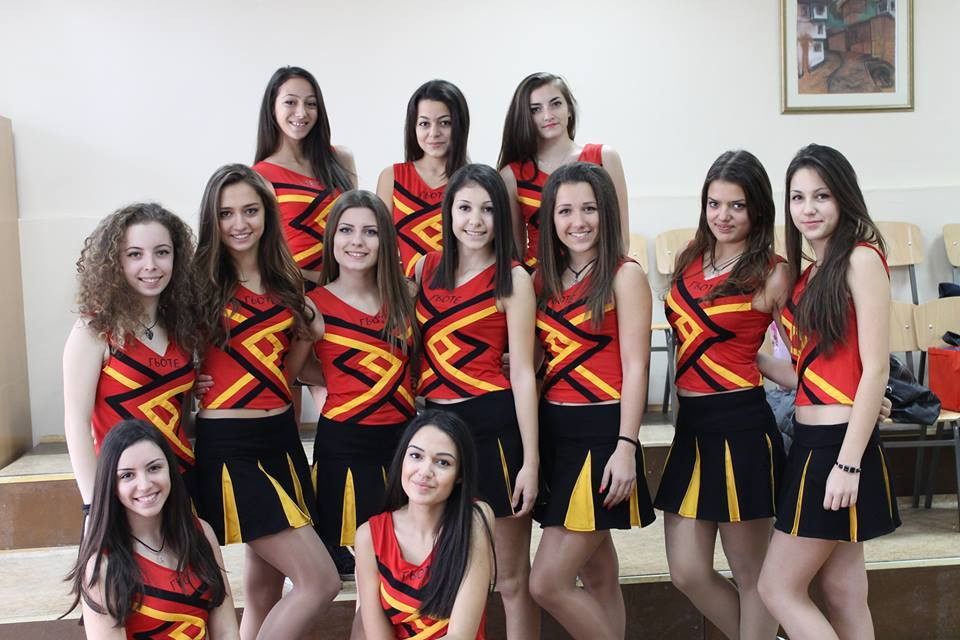
\includegraphics[width=6.1in]{./Magoretki/M.jpg}
\end{center}

\closearticle
